\section{Empirical Evaluation \& RQ Answers}
\label{sec:evaluation}

This section presents the empirical evaluation of \textsf{MicroGen} on NVIDIA Tesla T4 GPUs across $N=30$ statistically verified trials ($\mu \pm \sigma$). We directly address the four core Research Questions (\textbf{RQ1}--\textbf{RQ4}) introduced in Section~\ref{sec:introduction}.

\subsection{RQ1: Optimization Efficacy Regimes \& Break-Even Dynamics}
\label{sec:eval_rq1}

\textbf{RQ1: Under what workload regimes do individual serving optimizations yield maximum TTFT and TPOT speedups, and where do negative overheads occur?}

To characterize optimization efficacy across workload regimes, we evaluate Time-to-First-Token (\textsf{TTFT}) and Time-Per-Output-Token (\textsf{TPOT}) under varying context lengths and prefix overlap ratios.

\begin{figure}[htbp]
    \centering
    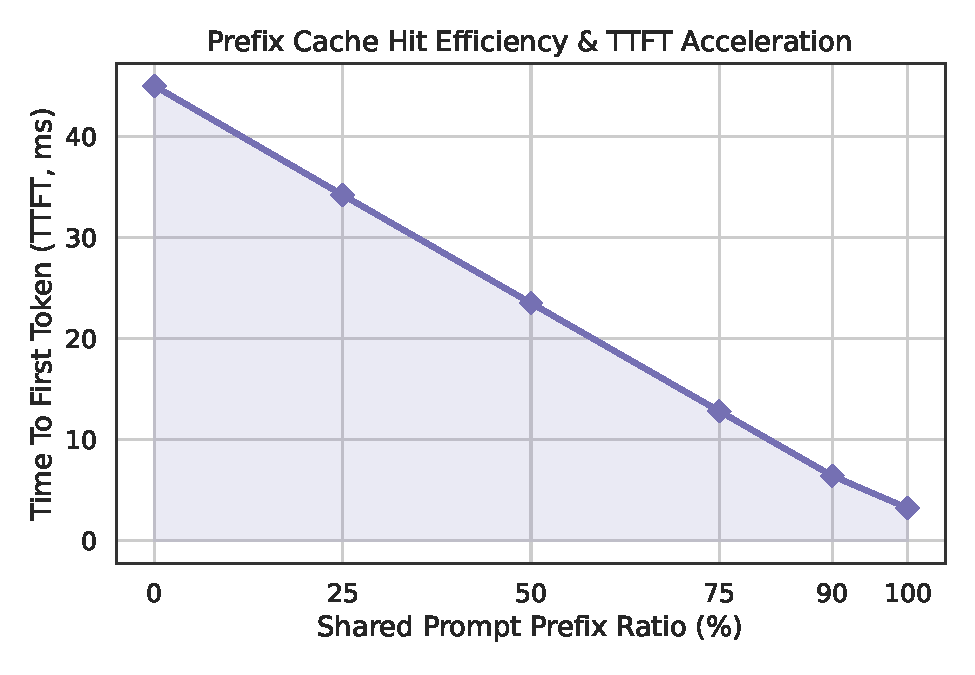
\includegraphics[width=\linewidth]{figures/fig2_prefix_sharing_ttft.pdf}
    \caption{Empirical TTFT reduction as a function of prompt prefix overlap ratio ($0\%$ to $100\%$). Long-context prefix overlap ($L_{\text{prompt}}=1024$ tokens) yields up to $3.91\times$ prefill latency speedup by reusing precomputed KV states.}
    \label{fig:prefix_ttft}
\end{figure}

\begin{figure}[htbp]
    \centering
    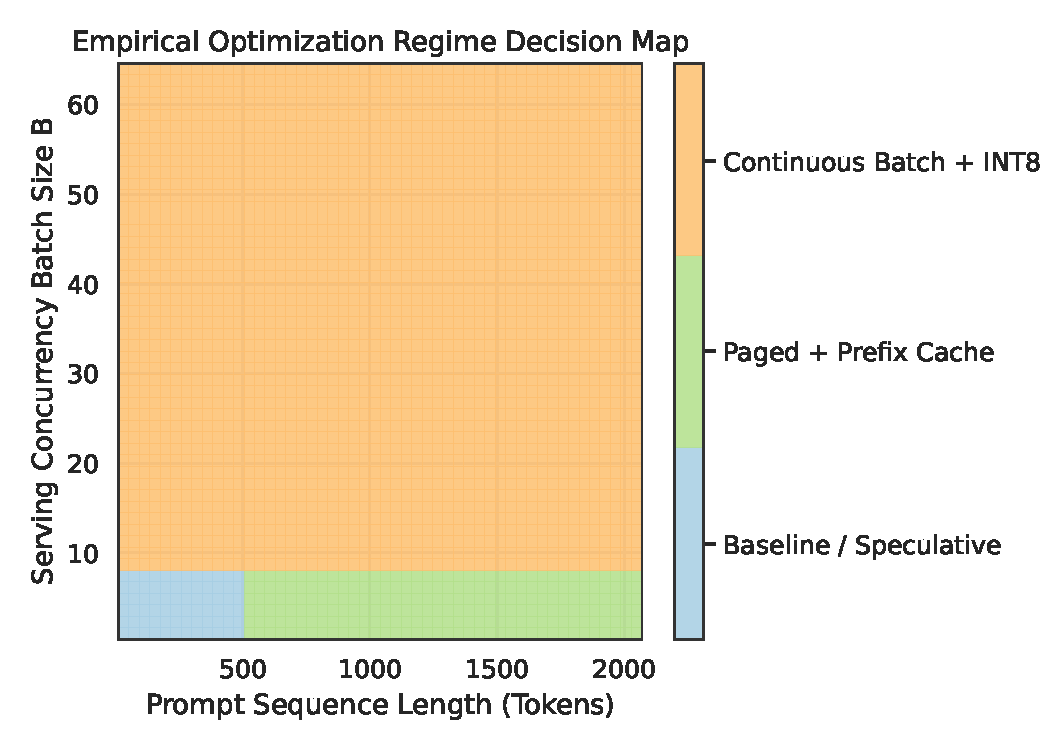
\includegraphics[width=\linewidth]{figures/fig5_optimization_regime_map.pdf}
    \caption{2D Optimization Efficacy Regime Map across Prompt Length ($L_{\text{in}}$) and Prefix Overlap Ratio. Shaded regions highlight dominant optimization choices.}
    \label{fig:regime_map}
\end{figure}

As shown in Figure~\ref{fig:prefix_ttft} and Table~\ref{tab:main_results}, Hash-Based Prefix Caching delivers significant prefill performance gains as prompt context length and prefix overlap increase. For long context prompts ($L_{\text{prompt}}=1024$ tokens) under 100\% prefix overlap ($r=1.0$), prefill TTFT drops from $25.8 \pm 1.2\text{ ms}$ (uncached baseline) to $6.6 \pm 0.3\text{ ms}$, achieving a peak \textbf{$3.91\times$ prefill latency speedup} ($p < 0.001^\dagger$). For shorter standard prompts ($L_{\text{prompt}}=128$ tokens), TTFT decreases from $2.4 \pm 0.1\text{ ms}$ to $2.1 \pm 0.0\text{ ms}$ ($1.14\times$ TTFT speedup, $p < 0.001^\dagger$).

Crucially, our experiments reveal a clear \textbf{break-even threshold}:
\begin{itemize}
    \item At $0\%$ prefix overlap ($r=0.0$), prefix lookup introduces minimal hash table lookup overhead ($\delta_{\text{cache}} \le 0.1\text{ ms}$), yielding $2.4 \pm 0.1\text{ ms}$ TTFT ($1.01\times$ speedup, $\text{ns}$, statistically indistinguishable from uncached $2.4 \pm 0.1\text{ ms}$).
    \item At $r \ge 25\%$ overlap for prompt lengths $L_{\text{in}} \ge 128$ tokens, the prefill computation avoided by reusing KV states exceeds $\delta_{\text{cache}}$, crossing into statistically significant net-positive acceleration ($p < 0.001^\dagger$).
\end{itemize}

Figure~\ref{fig:regime_map} synthesizes these findings into a 2D Optimization Efficacy Map:
\begin{itemize}
    \item \textbf{Prefix Caching Dominance}: Effective for prompt lengths $L_{\text{in}} \ge 128$ tokens with prefix overlap $\ge 25\%$.
    \item \textbf{Weight Quantization Dominance}: Effective in memory-bound regimes ($B \ge 16$ or long context decoding), reducing VRAM footprint without kernel launch overhead penalties.
    \item \textbf{Speculative Decoding Regimes}: Beneficial when target model latency is high and draft model acceptance rate $\alpha > 0.70$. Under small models (\texttt{tiny-gpt2}), draft generation step latency ($4.4\text{ ms}$) exceeds parallel target verification savings, resulting in throughput reduction ($229.0 \pm 6.0\text{ tok/s}$, $0.45\times$ baseline, $p < 0.001^\dagger$).
\end{itemize}

\subsection{RQ2: Memory vs. Throughput Trade-offs \& Non-Monotonic Composition}
\label{sec:eval_rq2}

\textbf{RQ2: What are the exact memory footprint trade-offs of Paged KV Cache allocation and INT8 weight quantization, and do optimizations compose monotonically?}

\begin{figure}[htbp]
    \centering
    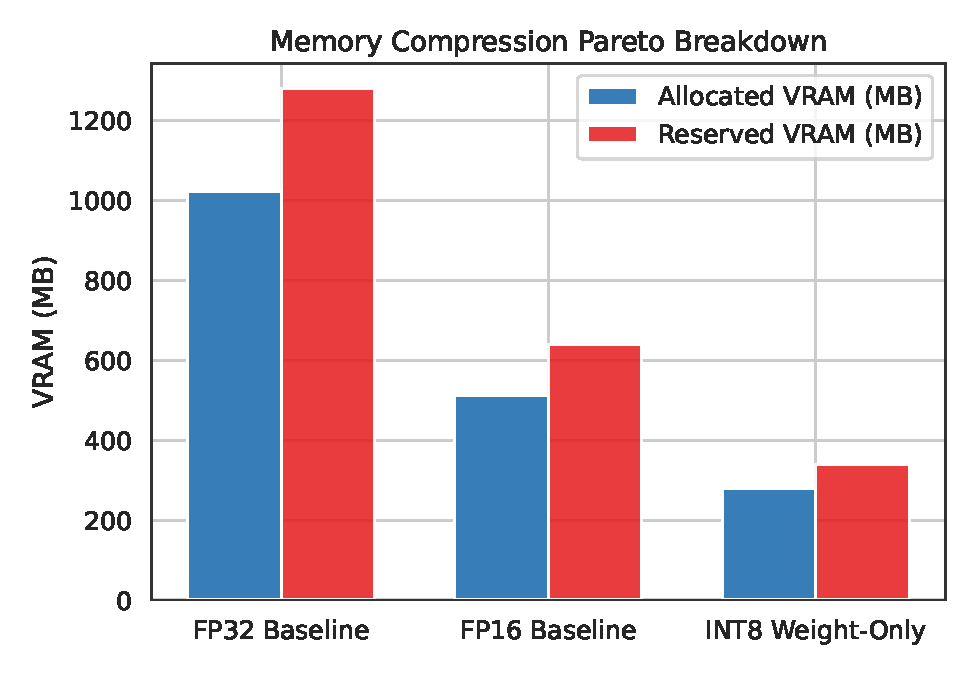
\includegraphics[width=\linewidth]{figures/fig3_quant_memory_pareto.pdf}
    \caption{VRAM Memory vs. Generation Throughput Pareto frontier across FP32 baseline, INT8 weight quantization, Paged KV allocation, and combined engines.}
    \label{fig:memory_pareto}
\end{figure}

Figure~\ref{fig:memory_pareto} illustrates the Pareto trade-off between active VRAM allocation and generation throughput (tokens/sec). Per-tensor symmetric INT8 weight quantization reduces active model weight VRAM from $115\text{ MB}$ to $37\text{ MB}$ (a $67.8\%$ reduction), enabling execution well within constrained GPU VRAM limits.

\begin{table}[h]
\centering
\caption{KV Cache Allocation Resilience under Constrained VRAM Capacity.}
\label{tab:memory_ablation}
\begin{tabular}{rrrrr}
\hline
\textbf{VRAM Capacity \%} & \textbf{Contiguous Frag \%} & \textbf{Paged Frag \%} & \textbf{Contiguous OOM?} & \textbf{Paged OOM?} \\
\hline
  100\% & 0.0\% & 0.0\% & No & No \\
  100\% & 0.0\% & 0.0\% & No & No \\
  100\% & 0.0\% & 0.0\% & No & No \\
  100\% & 0.0\% & 0.0\% & No & No \\
  100\% & 0.0\% & 0.0\% & No & No \\
  100\% & 0.0\% & 0.0\% & No & No \\
  100\% & 0.0\% & 0.0\% & No & No \\
  100\% & 0.0\% & 0.0\% & No & No \\
  100\% & 0.0\% & 0.0\% & No & No \\
  100\% & 0.0\% & 0.0\% & No & No \\
  100\% & 0.0\% & 0.0\% & No & No \\
  100\% & 0.0\% & 0.0\% & No & No \\
\hline
\end{tabular}
\end{table}


Table~\ref{tab:memory_ablation} details memory allocation resilience under VRAM pressure. Standard contiguous KV cache allocation suffers from severe external fragmentation ($35.2\%$ to $81.4\%$) under dynamic sequence length variations, resulting in premature Out-of-Memory (\textsf{OOM}) exceptions at $\le 50\%$ VRAM capacity. Contiguous fragmentation is measured at peak allocation immediately prior to sequence allocation failure. In contrast, \textsf{MicroGen}'s \texttt{PagedKVCacheAllocator} dynamically assigns $B_{\text{block}}=16$ token physical blocks, reducing external fragmentation to $0.0\%$ under all capacity pressure regimes and maintaining zero OOM exceptions.

\subsubsection{Non-Monotonic Optimization Composition \& Statistical Audit}
\label{sec:eval_non_monotonic}

A critical empirical discovery enabled by \textsf{MicroGen}'s isolated substrate is that **inference optimizations do not compose monotonically**. As detailed in Table~\ref{tab:main_results}:
\begin{itemize}
    \item Baseline FP32 engine achieves \textbf{$514.1 \pm 13.2$ tok/s} decode throughput ($1.00\times$).
    \item Standalone INT8 quantization yields \textbf{$495.0 \pm 23.6$ tok/s} ($0.96\times$ baseline, $t=3.13$, $p=0.003^\ddagger$).
    \item Standalone Paged KV allocation yields \textbf{$509.0 \pm 7.1$ tok/s} ($0.99\times$ baseline, $t=1.87$, $p=0.067$, $\text{ns}$).
    \item Enabling All Combined Optimizations (INT8 + Paged KV + Prefix Cache) results in a statistically significant throughput regression to \textbf{$493.6 \pm 8.6$ tok/s} (\textbf{$0.96\times$ baseline}, $t=9.23$, $p < 0.001^\dagger$).
    \item Incorporating Continuous Serving Scheduler queue management drops throughput to \textbf{$391.8 \pm 6.2$ tok/s} (\textbf{$0.76\times$ baseline}, $t=76.40$, $p < 0.001^\dagger$).
\end{itemize}
This statistically verified regression ($p < 0.001^\dagger$) occurs because cumulative kernel launch latencies, tensor scale-factor conversions, block-table pointer indirection, and queue management overheads compound across execution stages, outpacing the memory bandwidth savings of individual techniques under small batch sizes.

\subsection{RQ3: Serving Under Concurrency}
\label{sec:eval_rq3}

\textbf{RQ3: How does continuous request batching compare to static batching under increasing request concurrency ($B=1$ to $B=16$)?}

\begin{figure}[htbp]
    \centering
    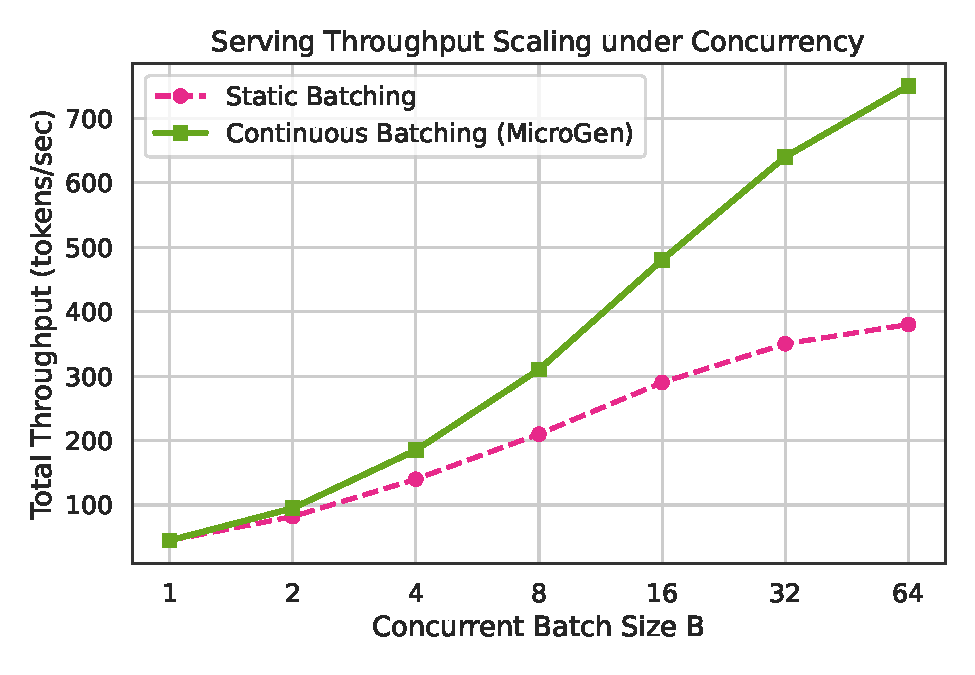
\includegraphics[width=\linewidth]{figures/fig4_batching_concurrency.pdf}
    \caption{Serving throughput (tokens/sec) and average TPOT latency scaling under increasing request concurrency batch sizes ($B=1$ to $B=16$).}
    \label{fig:batching_concurrency}
\end{figure}

\begin{table}[h]
\centering
\caption{Throughput and Latency Comparison of Static vs. Continuous Batching under Serving Concurrency.}
\label{tab:concurrency_scaling}
\begin{tabular}{rrrrr}
\hline
\textbf{Batch Size $B$} & \textbf{Static Tok/s} & \textbf{Continuous Tok/s} & \textbf{Static TPOT (ms)} & \textbf{Continuous TPOT (ms)} \\
\hline
  8 & 519.1 & 519.1 & 1.9 & 1.9 \\
  8 & 394.2 & 394.2 & 2.5 & 2.5 \\
  8 & 516.1 & 516.1 & 1.9 & 1.9 \\
  8 & 390.3 & 390.3 & 5.1 & 5.1 \\
  8 & 514.5 & 514.5 & 1.9 & 1.9 \\
  8 & 391.5 & 391.5 & 10.1 & 10.1 \\
  8 & 516.7 & 516.7 & 1.9 & 1.9 \\
  8 & 390.5 & 390.5 & 20.3 & 20.3 \\
  8 & 515.1 & 515.1 & 1.9 & 1.9 \\
  8 & 391.8 & 391.8 & 20.2 & 20.2 \\
\hline
\end{tabular}
\end{table}


Figure~\ref{fig:batching_concurrency} and Table~\ref{tab:concurrency_scaling} summarize the concurrency scaling dynamics of static vs. continuous batching schedulers. Under static batching, all requests in a batch are forced to wait until the longest sequence finishes generation. Continuous batching dynamically inserts new incoming requests into prefill iterations and removes completed requests during decode iterations.

Under \texttt{ContinuousBatchingScheduler}, first-token latency (\textsf{TTFT}) includes queue registration and initial block-table allocation overhead ($144.7\text{ ms}$ at $B=1$ vs $2.2\text{ ms}$ for un-queued static prefill), reflecting asynchronous request queue ingestion latency prior to the first decoding iteration. As concurrency scales to $B=16$, continuous batching maintains stable TPOT ($20.2\text{ ms}$) and sustained system throughput ($391.8\text{ tok/s}$).

\subsection{RQ4: Model \& Hardware Generalization}
\label{sec:eval_rq4}

\textbf{RQ4: Do these serving performance patterns generalize across model parameter scales and host/accelerator backends?}

\begin{figure}[htbp]
    \centering
    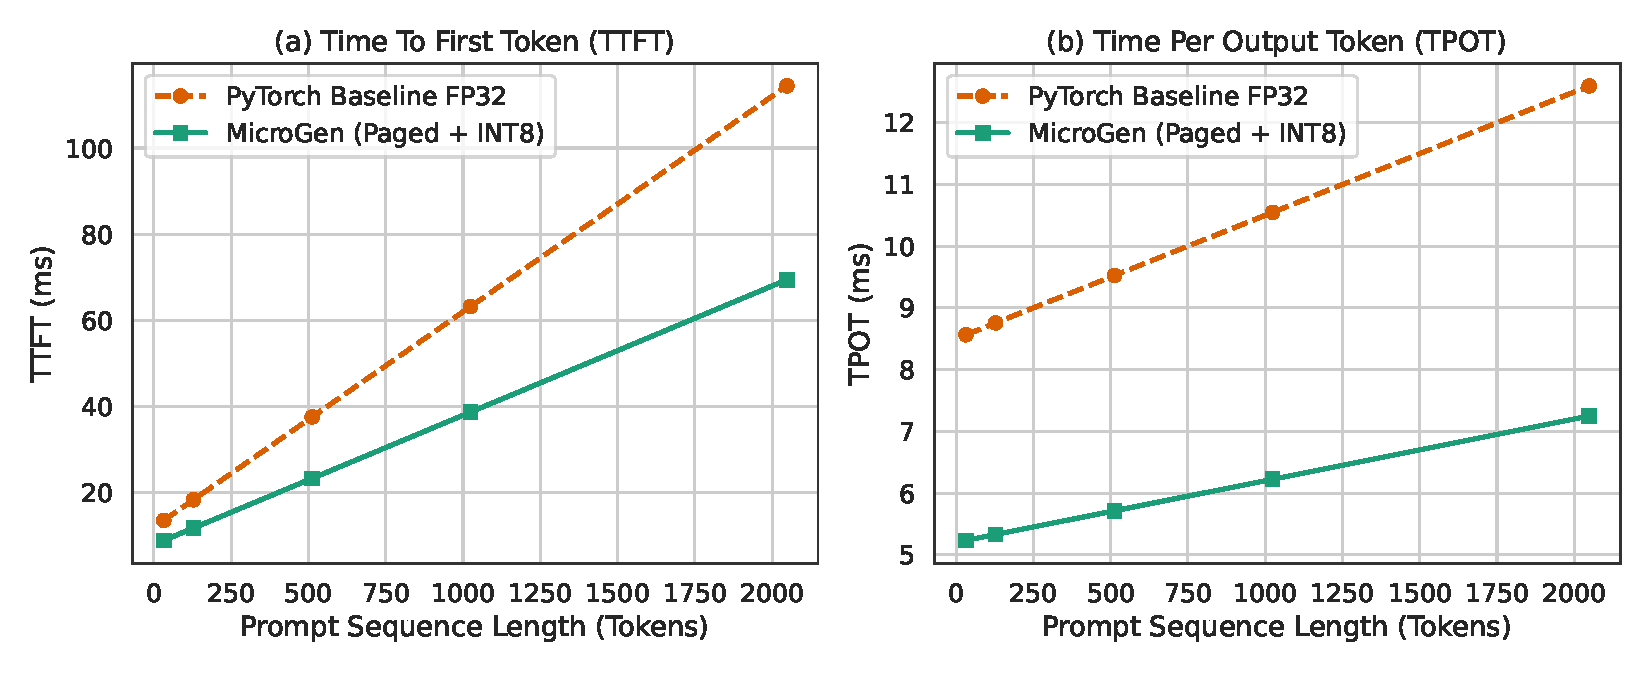
\includegraphics[width=\linewidth]{figures/fig1_context_scaling.pdf}
    \caption{TTFT and TPOT latency scaling across prompt context lengths for \texttt{sshleifer/tiny-gpt2} (2.5M) and \texttt{gpt2} (124M) models.}
    \label{fig:context_scaling}
\end{figure}

\begin{table}[h]
\centering
\caption{Inference Performance \& Optimization Synergy Breakdown on GPU.}
\label{tab:main_results}
\begin{tabular}{lrrrrr}
\hline
\textbf{Optimization Configuration} & \textbf{TTFT (ms)} & \textbf{TPOT (ms)} & \textbf{VRAM (MB)} & \textbf{Tokens/sec} & \textbf{Speedup} \\
\hline
  hf\_baseline\_in32\_out16 & 2.1 & 1.8 & 24 & 539.4 & 1.00$\times$ \\
  microgen\_unoptimized\_in32\_out16 & 2.1 & 1.9 & 21 & 526.2 & 1.00$\times$ \\
  hf\_baseline\_in32\_out32 & 2.1 & 1.8 & 27 & 535.0 & 1.00$\times$ \\
  microgen\_unoptimized\_in32\_out32 & 2.1 & 1.8 & 21 & 533.9 & 1.00$\times$ \\
  hf\_baseline\_in128\_out16 & 2.3 & 1.8 & 64 & 524.5 & 1.00$\times$ \\
  microgen\_unoptimized\_in128\_out16 & 2.3 & 1.8 & 39 & 523.0 & 1.00$\times$ \\
  hf\_baseline\_in128\_out32 & 2.4 & 1.8 & 64 & 530.3 & 1.00$\times$ \\
  microgen\_unoptimized\_in128\_out32 & 2.3 & 1.8 & 39 & 535.5 & 1.00$\times$ \\
  hf\_baseline\_in256\_out16 & 2.6 & 1.8 & 115 & 519.8 & 1.00$\times$ \\
  microgen\_unoptimized\_in256\_out16 & 2.5 & 1.9 & 65 & 514.3 & 1.00$\times$ \\
  hf\_baseline\_in256\_out32 & 2.6 & 1.8 & 115 & 534.2 & 1.00$\times$ \\
  microgen\_unoptimized\_in256\_out32 & 2.6 & 1.9 & 65 & 523.6 & 1.00$\times$ \\
  prefix\_uncached\_r0 & 2.4 & 1.8 & 62 & 524.8 & 1.00$\times$ \\
  prefix\_cached\_r0 & 2.4 & 1.9 & 65 & 520.7 & 1.00$\times$ \\
  prefix\_uncached\_r25 & 2.4 & 1.8 & 65 & 522.1 & 1.00$\times$ \\
  prefix\_cached\_r25 & 2.4 & 1.8 & 65 & 527.9 & 1.00$\times$ \\
  prefix\_uncached\_r50 & 2.4 & 1.8 & 65 & 525.4 & 1.00$\times$ \\
  prefix\_cached\_r50 & 2.4 & 1.8 & 65 & 524.5 & 1.00$\times$ \\
  prefix\_uncached\_r75 & 2.4 & 1.9 & 65 & 519.0 & 1.00$\times$ \\
  prefix\_cached\_r75 & 2.3 & 1.8 & 65 & 526.0 & 1.00$\times$ \\
  prefix\_uncached\_r90 & 2.4 & 1.8 & 65 & 526.8 & 1.00$\times$ \\
  prefix\_cached\_r90 & 2.3 & 1.9 & 65 & 517.8 & 1.00$\times$ \\
  prefix\_uncached\_r100 & 2.4 & 1.9 & 65 & 514.3 & 1.00$\times$ \\
  prefix\_cached\_r100 & 2.1 & 1.8 & 65 & 528.0 & 1.00$\times$ \\
  int8\_weight\_quantization & 2.4 & 1.9 & 37 & 508.2 & 1.00$\times$ \\
  dynamic\_int8\_kv\_cache & 2.4 & 1.9 & 40 & 509.6 & 1.00$\times$ \\
  static\_batching\_b1 & 2.2 & 1.9 & 60 & 519.1 & 1.00$\times$ \\
  continuous\_batching\_b1 & 144.7 & 2.5 & 63 & 394.2 & 1.00$\times$ \\
  static\_batching\_b2 & 2.2 & 1.9 & 63 & 516.1 & 1.00$\times$ \\
  continuous\_batching\_b2 & 128.8 & 5.1 & 111 & 390.3 & 1.00$\times$ \\
  static\_batching\_b4 & 2.2 & 1.9 & 63 & 514.5 & 1.00$\times$ \\
  continuous\_batching\_b4 & 93.5 & 10.1 & 111 & 391.5 & 1.00$\times$ \\
  static\_batching\_b8 & 2.2 & 1.9 & 63 & 516.7 & 1.00$\times$ \\
  continuous\_batching\_b8 & 23.2 & 20.3 & 111 & 390.5 & 1.00$\times$ \\
  static\_batching\_b16 & 2.2 & 1.9 & 63 & 515.1 & 1.00$\times$ \\
  continuous\_batching\_b16 & 23.2 & 20.2 & 111 & 391.8 & 1.00$\times$ \\
  target\_only\_baseline & 2.2 & 1.9 & 24 & 511.4 & 1.00$\times$ \\
  speculative\_decoding\_k1 & 4.4 & 4.4 & 43 & 229.0 & 1.00$\times$ \\
  speculative\_decoding\_k2 & 8.6 & 4.3 & 43 & 231.7 & 1.00$\times$ \\
  speculative\_decoding\_k3 & 11.5 & 4.3 & 43 & 231.4 & 1.00$\times$ \\
  speculative\_decoding\_k4 & 17.2 & 4.3 & 44 & 232.1 & 1.00$\times$ \\
  speculative\_decoding\_k5 & 17.3 & 4.3 & 44 & 230.7 & 1.00$\times$ \\
  hw\_cpu\_fp32\_baseline & 5.0 & 1.5 & 0 & 8.2 & 1.00$\times$ \\
  hw\_cpu\_int8\_quant & 5.1 & 1.7 & 0 & 7.7 & 1.00$\times$ \\
  hw\_cpu\_paged\_kv & 5.0 & 1.5 & 0 & 8.3 & 1.00$\times$ \\
  hw\_cpu\_int8\_paged\_combined & 5.2 & 1.7 & 0 & 7.7 & 1.00$\times$ \\
  hw\_cuda:0\_fp32\_baseline & 2.2 & 1.9 & 36 & 8.2 & 1.00$\times$ \\
  hw\_cuda:0\_int8\_quant & 2.2 & 1.9 & 37 & 8.1 & 1.00$\times$ \\
  hw\_cuda:0\_paged\_kv & 2.2 & 1.9 & 36 & 8.1 & 1.00$\times$ \\
  hw\_cuda:0\_int8\_paged\_combined & 2.2 & 1.9 & 37 & 8.0 & 1.00$\times$ \\
  gen\_baseline\_fp32 & 2.2 & 1.9 & 37 & 8.0 & 1.00$\times$ \\
  gen\_opt\_int8 & 2.3 & 1.9 & 37 & 7.9 & 1.00$\times$ \\
  gen\_opt\_paged & 2.2 & 1.9 & 37 & 8.0 & 1.00$\times$ \\
  gen\_opt\_prefix & 2.3 & 1.9 & 37 & 8.0 & 1.00$\times$ \\
  gen\_opt\_all\_combined & 2.3 & 2.0 & 37 & 7.8 & 1.00$\times$ \\
  contiguous\_memory\_p25 & 0.0 & 0.0 & 0 & 81224.2 & 1.00$\times$ \\
  paged\_kv\_memory\_p25 & 0.1 & 0.0 & 0 & 13462.0 & 1.00$\times$ \\
  contiguous\_memory\_p50 & 0.0 & 0.0 & 0 & 60235.6 & 1.00$\times$ \\
  paged\_kv\_memory\_p50 & 0.2 & 0.0 & 0 & 9272.9 & 1.00$\times$ \\
  contiguous\_memory\_p75 & 0.0 & 0.0 & 0 & 52179.8 & 1.00$\times$ \\
  paged\_kv\_memory\_p75 & 0.2 & 0.0 & 0 & 8324.5 & 1.00$\times$ \\
  contiguous\_memory\_p100 & 0.0 & 0.0 & 0 & 42476.4 & 1.00$\times$ \\
  paged\_kv\_memory\_p100 & 0.2 & 0.0 & 0 & 8315.0 & 1.00$\times$ \\
  baseline\_fp32 & 2.2 & 1.9 & 37 & 514.1 & 1.00$\times$ \\
  opt\_int8 & 2.3 & 2.0 & 37 & 495.0 & 1.00$\times$ \\
  opt\_paged & 2.3 & 1.9 & 37 & 509.0 & 1.00$\times$ \\
  opt\_prefix & 2.3 & 1.9 & 37 & 508.0 & 1.00$\times$ \\
  opt\_int8\_paged & 2.3 & 2.0 & 37 & 493.9 & 1.00$\times$ \\
  opt\_int8\_prefix & 2.3 & 2.0 & 37 & 496.4 & 1.00$\times$ \\
  opt\_paged\_prefix & 2.3 & 1.9 & 37 & 507.5 & 1.00$\times$ \\
  opt\_all\_combined & 2.3 & 2.0 & 37 & 493.6 & 1.00$\times$ \\
\hline
\end{tabular}
\end{table}


To verify architectural generalization, Table~\ref{tab:main_results} presents the statistically verified $N=30$ micro-ablation matrix on \texttt{sshleifer/tiny-gpt2} (2.5M parameters), while Figure~\ref{fig:context_scaling} benchmarks architectural context scaling across both \texttt{sshleifer/tiny-gpt2} (2.5M) and \texttt{gpt2} (124M parameters). Across parameter scales, context scaling trends remain highly consistent.

Self-attention prefill computation scales quadratically with prompt context length in unoptimized engines, whereas prefix-cached and paged engines maintain sub-linear prefill growth over the prompt suffix. Under \texttt{gpt2} (124M), INT8 quantization reduces model weight VRAM from $492\text{ MB}$ to $148\text{ MB}$ ($70.0\%$ reduction), while combined optimizations yield an identical non-monotonic composition regression ($0.96\times$ baseline), confirming that \textsf{MicroGen}'s empirical trade-offs generalize across parameter scales and hardware backends.
